\documentclass[11pt]{article}
\usepackage{amsmath}
\usepackage{amssymb}
\usepackage{tikz}
\usepackage{wrapfig}
\usepackage{caption}
\usepackage{graphicx}
\usepackage{subcaption}
\usetikzlibrary{arrows}
\title{\textbf{Proposal for a socialist blockchain system}}
\author{Stachanov Developer Collective}
\date{}
\begin{document}

\maketitle
\tableofcontents

\section{Introduction}

In the past years blockchain technology has been utilized as a mean for digital currency and contracts. Even if most of the financial industry is still sceptical (mainly because they don't understand the technology) blockchain has gained traction in a significant part of the tech community. However, looking at the assumptions build into Bitcoin and other blockchain currencies, we receive the impression that the goal is a right-wing libertarian utopia, in which every aspect of life is modeled as a payable commodity.

We are not the first to notice. Last year people from GNU proposed GNU Taler, a currency that is taxable, but claims to have buyer privacy protection. This could be called a social democratic approach, that tries to include the welfare state (or what's left of it) into decentralized money transfer. Other projects like Grantcoin (now Manna) try to put "ethical consumption" onto the blockchain. 

Even if we are somewhat sympathetic to such approaches, we think they are false middle grounds and built on wrong assumptions. Looking at GNU Taler and the Keynesian Left we find the naive belief that the nation state could still "turn around" and "rediscover it's true purpose to serve the people". We see this as a fatal melancholic nostalgia, that keeps the Left frozen and powerless. We must recognize, that capital as a movement of surplus generation has transcended the nation state as it transcended the divided European principalities in the 19th century. There is to turning back. The enthusiasm about blockchain currencies is a superstructure symptom of this economic fact. We also reject the idea of left fukayamism, that wants a fairer, greener, more ethical capitalism. All these concepts managed to do was to generate a feeling of guilt-free consumption for the upper middle class. When we think of a good society we don't think of it as "more Wholefood Markets".

In this paper we propose a more radical solution, a decentralized socialist society that aims to replace market economy completely without falling back to the state planning bureaucracy of the old soviet republics. Instead of contract relations between private property owners, we model production and good transfer as a simple relation: The relation of individuals to society.

In this model individuals contribute to societal wealth by giving part of their time to work for society. The spent time is registered on the blockchain and fulfills two functions: First it is used to tag products with the amount of time that was needed to produce them, second it creates entitlements for individuals to appropriate wealth. In this paper we want to provide a sketch on how such a system could work.

\begin{figure}
\centering

\begin{minipage}[l]{0.4\textwidth}
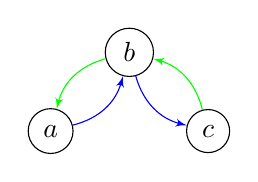
\begin{tikzpicture}

\tikzset{vertex/.style = {shape=circle,draw,minimum size=1.5em}}
\tikzset{edge/.style = {->,> = latex'}}
% vertices
\node[vertex] (a) at  (2,0) {$a$};
\node[vertex] (b) at  (3,1) {$b$};
\node[vertex] (c) at  (4,0) {$c$};
%edges
\tikzset{edge/.style = {->, green, > = latex'}}
\draw[edge] (b) to[bend right] (a);
\draw[edge] (c) to[bend right] (b);
\tikzset{edge/.style = {->, blue, > = latex'}}
\draw[edge] (b) to[bend right] (c);
\draw[edge] (a) to[bend right] (b);


\end{tikzpicture}
\caption{private exchange between property owners. Money (green) gets exchanged with services and commodities (blue)}
\end{minipage}
\hfill\vline\hfill
\begin{minipage}[r]{0.4\textwidth}
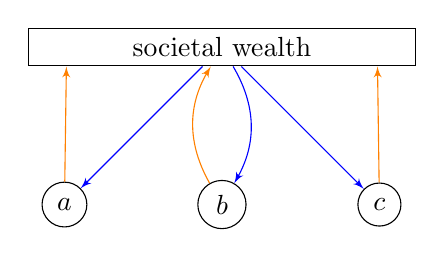
\begin{tikzpicture}
\tikzset{vertex/.style = {shape=rectangle,draw,minimum width=14em}}
\node[vertex] (s) at  (0,0) {    societal wealth    };
\tikzset{vertex/.style = {shape=circle,draw,minimum size=1.5em}}
\tikzset{edge/.style = {->,> = latex'}}
% vertices
\node[vertex] (a) at  (-2,-2) {$a$};
\node[vertex] (b) at  (0,-2) {$b$};
\node[vertex] (c) at  (2,-2) {$c$};
%edges
\tikzset{edge/.style = {->, orange, > = latex'}}
\draw[edge] (a) to[xshift=-40em] (s);
\draw[edge] (b) to[bend left] (s);
\draw[edge] (c) to[xshift=40em] (s);

\tikzset{edge/.style = {->, blue, > = latex'}}
\draw[edge] (s) to[] (a);
\draw[edge] (s) to[bend left] (b);
\draw[edge] (s) to[] (c);


\end{tikzpicture}
\caption{carrying out work for society (orange) and individual appropriation of commodities and services (blue).}
\end{minipage}


\end{figure}




\section{Collectives and economic subsystems}

\emph{Collectives} are the frame of reference in which production takes place. They are steady or loose associations of people, that do work in the broadest sense, be it producing commodities, providing a service, doing research, planing or educating. 

For every timespan someone is working in a collective, the collective registers workloads, that can be transformed into labor coupons at a later time. These coupons can then be used by the individual worker to appropriate commodities or services from societal wealth.

Since coupons need to represent actual work, collectives must trust each other, that workloads are actually rendered. This is why a system of mutual checks is provided, which guarantees that coupons created by workloads of collective A can only be used to appropriate wealth produced by collective B, when there is trust between them. The same principle is applied when commodities or means of productions are transfered. If A produces for collective B it must be sure that B does not privately consume the provided goods, but continues processing them or provides them for consumers. Thus A can only transfer goods to B if there is trust between them.

Trust between collectives creates (potentially) several trust graphs on the chain, similar to PGP's web of trust. Each connected graph forms an economic subsystem in which commodity transfer and coupon usage is possible.

\subsection{The trust graph}

We propose a rather simple model of trust, in which trust is symmetric and transitive. These properties are needed to build economic subsystems in which every collective is treated equal. 

Let $G=(V, E)$ be an undirected trust graph where $V$ represents the collectives and $E$ the trust connections between them.

\begin{itemize}
\item We say that $v_1$ and $v_2$ established \emph{strong trust} in each other when $\{v_1, v_2\} \in E$
\item We say that $v_1$ and $v_2$ established \emph{weak trust} in each other, when there is a path from $v_1$ to $v_2$ in $G$
\end{itemize}

On the blockchain \emph{strong trust} is established by a mutual signature of two collectives. We define the economic subsystem as follows:

\begin{itemize}
\item Collectives $v_1$ and $v_2$ can transfer goods to each other, when they established \emph{strong trust}
\item An individual can use a work coupon generated from a workload registered at $v_1$ at a dispatcher collective $v_2$, when $v_1$ and $v_2$ established \emph{weak trust}
\end{itemize}

The rationale behind the different treatment of inter-collective good transfer and good transfer from dispatchers to individuals is that in the second case only small amounts are transfered and cheating doesn't carry as much weight as in the first case, where potentially thousands of products or valuable means of productions change the owner.

There is also a technical reason: If only \emph{strong trust} between every collective would be sufficient we would (under the assumption that we want every collective to recognize each others coupons) have a memory complexity of $O(|V|!$) which is simply not practical. Also ideally "real" trust is only established, when collectives know each other somewhat personally, which would be impossible on a global production scale when every collective would need to know every other collective.

\paragraph{Canceling trust relationships}

Trust relationships can also get cancelled by one of the original signers. This is implemented as a safeguard, if one collective cheats or a private key is lost. If cancelling a trust relationship decomposes the trust graph into two components, the system must make sure, that some kind of settlement between the two subsystems is reached in order to mantain the parity of labor coupons values and commodity values. 

\subsection{C2C Collectives vs C2I Collectives}

C2C and C2I stands for Collective-to-Collective and Collective-to-Individuals. C2C collectives produce for other collectives, while C2I collectives dispatch goods and services to individuals. C2I collectives can create special transactions that signify, that a product has been handed to (some) consumer. To protect privacy there is no link between a specific product and a labor coupon wallet in the appropriation process. The C2I collective must only make sure that the wallet owner deleted the appropriate amount of labor coupons (this can be done by smartcard terminals) and make a physical inventory from time to time.

\section{Transfer and management of resources}

Resources can be transfered between two collectives with a multi signature transaction. 

\subsection{Original appropriation}

After the physical appropriation of the means of production, collectives (typically the old workforce of a factory) can claim resources with a \emph{collectivization transaction}. From the blockchain's point of view these resources are created out of thin air, they lack production data and thus can not have a reliable value tag. That means using these resources adds zero value to the product. Of course this is a misreprentation, but it keeps the internal parity of coupons and commodity value inside the system intact. The necessary effect of this model is that, when production is increasingly registered on the chain, commodity values will increase until they reach their real height.
Collectivization transactions include a resource definition (type, amount, etc), the collective's public key and its signature. Collectivization transactions are also used for products acquired through extern trade. 

\subsection{Ownership transfer}

When resources are registered in the blockchain, they can change the owner. Change of ownership is done through a double signature transaction, one signature from the current owner collective, another from the future owner collective. The transaction also includes the resource definition.

\subsection{Write-offs}

Collectives can write off resources, when they are expired or broken. In order to write off a resource, the owner collective makes a transaction with a reason and a reference to the original ownership transaction. Write-off transactions \emph{can} represent wasted work, for example when a cold chain was broken or a mean of production broke before it's estimated expiration date. The value of wasted work is added to the labor coupon taxation (more on that later). If a mean of production lasts longer than estimated, a write-off can also trigger a \emph{decrease} in tax rate.

\section{Product definition}

\subsection{Product roles}

In every economy products can have two different roles: They can be either used consumptively or as a mean of production.
\begin{itemize}
\item \textbf{Consumptive use} completely transfers the original value to the output product. Suppose you would produce cookie dough by hand. The value of the cookie dough is the sum of the values of the ingredients plus the time you have spent to make them.\footnote{This is only partially correct. The example doesn't take into account, that the \emph{average} working time is added to the value. For a possible solution on this see 6.2}
\item \textbf{Use as mean of production} does \emph{not} transfer the complete value of the product to the output product. An oven does not transfer its complete value to every plate of cookies produced in it. Rather the value transfer depends on the durability of the oven. If the oven has a value of 30 hours and you can use it 3000 times before it becomes obsolete, the value transfer for each plate is $\frac{1}{100}$ hours. 
\end{itemize}

The value transfer model confronts us with a problem: Modern MoPs are not monolithic structures, but rather assembled from different parts, that have different durability. The easiest example would be a laptop. The laptop battery lasts maybe 2 years, while the laptop itself lasts (ideally) more than that. This means that the value transfer of the laptop (if used as MoP) can not be decribed by a single pair of value and durability alone, but needs at least two such pairs, one for the battery, one for the laptop without it. We therefor need to carefully define \emph{simple} and \emph{composite} products.

\subsection{Simple and composite products}

Let $\mathbb{T}$ be the set of available product types and $P=(T, E)$ with $T \subseteq \mathbb{T}$ a directed graph without a closed walk and with edges $E \subseteq T^2$. An edge $e=(t_1, t_2)$ in this graph means:

\begin{itemize}
\item $t_1$ needs $t_2$ as an input resource.
\item $t_1$ can be seperated in a way that $t_2$ is available as a single (not necessarily functional) product again
\end{itemize}

With this definition we now define simple and composite products. A simple product can not be seperated (or it does not make economic sense to do so). They are defined as $P=(\{t\}, \emptyset)$. Products created for \emph{consumption} (as defined above) should always be modeled as simple products. Information about composition is only needed, when a product acts as a mean of production.


We define the following functions on P:

\begin{itemize}
\item $c(t): T \rightarrow \mathcal{P}(T) $ maps a product element to its direct subelements:
\begin{equation}
c(t) = \{t_c | (t, t_c) \in E\}
\end{equation} 
\item $s(t): T \rightarrow \mathcal{P}(T)$ maps a product element to \emph{all} its subelements:
\begin{equation}
  s(t)=\begin{cases}
    \emptyset, & \text{if $c(t) = \emptyset$}\\
    \bigcup_{t_c \in c(t)} s(t_c) \cup c(t) & \text{otherwise}.
  \end{cases}
\end{equation}
\item $d(t): T \rightarrow \mathbb{N}$ maps product elements to their durability in minutes. It is defined as
\begin{equation}
  d(t)=\begin{cases}
    n, & \text{if $c(t) = \emptyset$}\\
    min\{d(t_c) | t_c \in c(t)\}, & \text{otherwise}.
  \end{cases}
\end{equation}
where n can be any number $\in \mathbb{N}$
\item $v(t) \rightarrow \mathbb{N}_0$ is the simple value of a product element measured in minutes.
\item $v^*(t) \rightarrow \mathbb{N}_0$ is the aggregated value of a product element in minutes and defined as:
\begin{equation}
  v^*(t)= v(t) + \sum_{t_s \in s(t)} v(t_s)
\end{equation}
\end{itemize}
To understand the model imagine we are assembling a computer from the following parts: A case, a mainboard, CPU, a RAM module, a hard drive. We have some basic information about the parts and the necessary utilities.

\begin{center}
  \begin{tabular}{ l | c | c | c | c | c }
    \hline
    description & t & $c(t)$ & $d(t)$ & $v(t)$ & $v^*(t)$ \\ \hline
    case & c & $\emptyset$ & $12*(356*24*60)$ & 200 & 200\\ \hline
    mainboard & m & $\emptyset$ & $12*(356*24*60)$ & 600 & 600\\ \hline
    CPU & p & $\emptyset$ & $9*(356*24*60)$ & 2500 & 2500\\ \hline
    RAM module & r & $\emptyset$ & $8*(356*24*60)$ & 700 & 700\\ \hline
    hard drive & h & $\emptyset$ & $5*(356*24*60)$ & 400 & 400\\ \hline
    heat paste & x & $\emptyset$ & $5*(356*24*60)$ & 30 & 30\\ \hline
    hard disk cable & y & $\emptyset$ & $10*(356*24*60)$ & 10 & 10\\ \hline
   
    \hline
  \end{tabular}
\end{center}


\begin{figure}
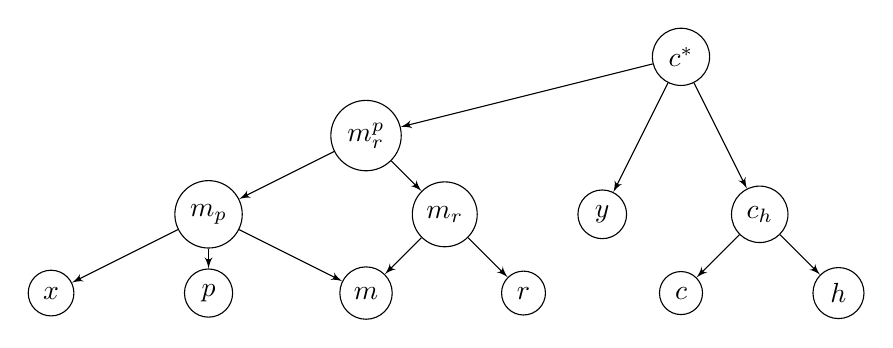
\begin{tikzpicture}
\centering
\tikzset{vertex/.style = {shape=circle,draw,minimum size=1.5em}}
\tikzset{edge/.style = {->,> = latex'}}
% vertices
\node[vertex] (a) at  (1,0) {$x$};
\node[vertex] (b) at  (3,1) {$m_{p}$};
\node[vertex] (c) at  (3,0) {$p$};
\node[vertex] (d) at  (5,0) {$m$};
\node[vertex] (e) at  (7,0) {$r$};
\node[vertex] (f) at  (6,1) {$m_r$};
\node[vertex] (g) at  (5,2) {$m^{p}_{r}$};
\node[vertex] (h) at  (9,0) {$c$};
\node[vertex] (i) at  (11,0) {$h$};
\node[vertex] (j) at  (10,1) {$c_{h}$};
\node[vertex] (k) at  (8,1) {$y$};
\node[vertex] (l) at  (9,3) {$c^*$};

%edges
\tikzset{edge/.style = {->, > = latex'}}
\draw[edge] (b) to[] (a);
\draw[edge] (b) to[] (c);
\draw[edge] (b) to[] (d);
\draw[edge] (f) to[] (e);
\draw[edge] (f) to[] (d);
\draw[edge] (g) to[] (f);
\draw[edge] (g) to[] (b);
\draw[edge] (j) to[] (i);
\draw[edge] (j) to[] (h);
\draw[edge] (l) to[] (k);
\draw[edge] (l) to[] (j);
\draw[edge] (l) to[] (g);
\end{tikzpicture}
\caption{Assembled product "Computer"}
\end{figure}

We now assemble CPU and mainboard to a new resource "Mainboard with CPU" using the heat paste. Suppose this assembly takes us 10 minutes. Then we insert the RAM module, which takes us 1 minute, creating a new product "Mainboard with RAM". At the same time someone else adds the harddrive to the case in 2 minutes.

We update our table accordingly:


\begin{center}
  \begin{tabular}{ l | c | c | c | c | c }
    \hline
    description & t & $c(t)$ & $d(t)$ & $v(t)$ & $v^*(t)$ \\ \hline
    mainboard with CPU & $m_{p}$ & $\{x, p, m\}$ & $5*(356*24*60)$ & 10 & 3140\\ \hline
    mainboard with RAM & $m_{r}$ & $\{m, r\}$ & $8*(356*24*60)$ & 1 & 1301
    \\ \hline
    case with harddrive & $c_{h}$ & $\{c, h\}$ & $5*(356*24*60)$ & 2 & 602
    \\ \hline
    \hline
  \end{tabular}
\end{center}

The rationale of setting $d(t)$ to the minimum durability value of its descendants now becomes clear. The work inserting the RAM becomes obsolete, once the RAM module or the mainboard becomes obsolete. Since the durability of the RAM is lesser than the durability of the mainboard, the durability of the assembly work is the durability of the RAM. 

We can now combine $m_p$ and $m_r$ to a product element "mainboard with CPU and RAM", which is purely virtual and doesn't need extra work.

\begin{center}
  \begin{tabular}{ l | c | c | c | c | c }
    \hline
    description & t & $c(t)$ & $d(t)$ & $v(t)$ & $v^*(t)$ \\ \hline
    board with CPU / RAM& $m_{r}^{p}$ & $\{m_{p}, m_{r}\}$ & $5*(356*24*60)$ & 0 & 3841  \end{tabular}
\end{center}

After that we add the mainboard to the case and connect the harddrive to the mainboard with a cable in 15 minutes. Again we calculate the values:

\begin{center}
  \begin{tabular}{ l | c | c | c | c | c }
    \hline
    description & t & $c(t)$ & $d(t)$ & $v(t)$ & $v^*(t)$ \\ \hline
    computer & $c^*$ & $\{m^{p}_{r}, c_{h}, y\}$ & $5*(356*24*60)$ & 15 & 4468  \end{tabular}
\end{center}

\subsection{Value transfer of composite means of productions}

Given the above definitions we can now define an additional function $\delta(t, k) : T \times \mathbb{N} \rightarrow \mathbb{N}$, that denotes the durability of a product element at a point in time k:

\begin{equation}
\delta(t, k) = max(d(t) - k, 0)
\end{equation}

and another function $\rho(t, k_1, k_2): T \times \mathbb{N} \times \mathbb{N} \rightarrow \mathbb{N}$ with $k_2 > k_1$ and the following definition:

\begin{equation}
\rho(t, k_1, k_2) = \frac{\delta(t, k_1) - \delta(t, k_2)}{d(t)}
\end{equation}

We can now define the value transfer $\theta(P, k_1, k_2)$ of a product $P=(T, E)$ between a time $k_1$ and $k_2$ with $k_1 < k_2$:

\begin{equation}
\theta(t, k_1, k_2) = \sum_{t \in T} \rho(t, k_1, k_2) * v(t)
\end{equation}

Let be $Y := (356*24*60)$ the minutes in a year. Let's suppose our computer runs for two years. We want to calculate how much value was transfered from our computer in the second year ($k_1 := 1Y, k_2 := 2Y$) to the products produced with it.

\begin{center}
  \begin{tabular}{ l | c | c | c | c | c | c | c}
    \hline
        t & $d(t)$ & $\delta(t, 1Y)$ & $\delta(t, 2Y)$ & $\rho(t, 1Y, 2Y)$ & $v(t)$ & $\rho(t, 1Y, 2Y) * v(t)$\\ \hline
    c & $12Y$ & $11Y$ & $10Y$ & $\frac{1}{12}$ & 200 & $\approx 17$ \\ \hline
    m & $12Y$ & $11Y$ & $10Y$ & $\frac{1}{12}$ & 600 & 50\\ \hline
    p & $9Y$ & $8Y$ & $7Y$ & $\frac{1}{9}$ & 2500 & $\approx 278$ \\ \hline
    r & $8Y$ & $7Y$ & $6Y$ & $\frac{1}{8}$ & 700 & $\approx 88$ \\ \hline
    h & $5Y$ & $4Y$ & $3Y$ & $\frac{1}{5}$ & 400 & 80\\ \hline
    x & $5Y$ & $4Y$ & $3Y$ & $\frac{1}{5}$ & 30 & 6\\ \hline
    y & $10Y$ & $9Y$ & $8Y$ & $\frac{1}{10}$ & 10 & 1 \\ \hline
    $m_{p}$ & $5Y$ & $5Y$ & $4Y$ & $\frac{1}{5}$ & 10 & 2\\ \hline
    $m_{r}$ & $8Y$ & $7Y$ & $6Y$ & $\frac{1}{8}$ & 1 & $\approx 1$ \\ \hline
    $c_{h}$ & $5Y$ & $4Y$ & $3Y$ & $\frac{1}{5}$ & 2 & $\approx 1$ \\ \hline
    $m^{p}_{r}$ & $5Y$ & $4Y$ & $3Y$ & $\frac{1}{5}$ & 2 & 0 \\ \hline
    $c^*$ & $5Y$ & $4Y$ & $3Y$ & $\frac{1}{5}$ & 15 & 3 \\ \hline
    \hline
  \end{tabular}
\end{center}

If we sum up all the values of the rightmost column we get the value transfer in minutes, which is roughly 530 minutes. Let's suppose we used the computer as a controller for robots in a car factory. Let's further assume we produced 500 000 cars in this year. Then the value transfer of the computer to each car is $\frac{530}{500 000} \approx 0.0016$ minutes.

\section{Production cycles}

A production cycle consists of multiple transaction types:

\begin{itemize}
\item \textbf{Order} Every production start needs an order transaction to refer to. Order transactions can refer other order transactions or can be self-appointed. Orders include a product definition, an amount, the ordering collective, a delivery time and a signature of the issuing collective. Order transactions can only be done between collectives which established \emph{strong trust} in each other.
\item \textbf{Order rejection} A collective can reject an order at any time. There should be a reason (such as over-capacity) attached to the transaction.  
\item \textbf{Value Estimation} If a collective decides to accept an order it broadcasts a value estimation to the chain.
\item \textbf{Production Start} A production start transaction initializes the production. After production start resources, means of production and workloads can be allocated. Production start transactions need to refer to a value estimation in a 1:1 relationship. In a later version of the system there should be an intermediate Production Vote transaction between Estimation and Production Start, when the estimated value exceeds a specific amount in order to democractically legitimize larger projects.

\item \textbf{Consumptive Resource Allocation} Collectives can allocate resources they own for the production process. The value of the resource gets completetly transfered to the end product.

\item \textbf{Workload Allocation} Workloads include an amount of time and a public key of a wallet. The amount of time gets fully transfered to the value of the end product.

\item \textbf{Mean of Production Allocation} The collective can allocate machines, that it owns for the production process. 

\item \textbf{Mean of Production Deallocation} The collective can deallocate a mean of production after it is not needed for the production anymore. Once a MoP is deallocated the value transfer to the end product can be calculated. This means, that before a Production Output transaction is issued, all MoPs must be deallocated.

\item \textbf{Production Output} In order to finalize a production cycle, collectives broadcast a Production Output transaction. Production output transactions can include multiple output product types. The system must make sure, that the complete value of the output equals the workloads, comsumptive resources and the value transfer of the used MoPs.
\end{itemize}

\section{Appropriation and commons production}

For every performed work time, a wallet holder can claim labor coupons, that in turn can be used to appropriate societal wealth. Labor coupons are not a currency. They can not be transfered or exchanged. If they are used for appropriation, they are \emph{deleted}. 

\subsection{Commons and exclusive goods}

Inside an economic subsystem, collectives should agree on product and service types, that are free (\emph{commons}) and ones, that require a proof of merit (\emph{exclusive}). When a product or service is labeled as a common, the workload time is substracted evenly from all labor coupons through taxation.

The common label can be added to orders, production starts, workload transactions, MoP allocations/deallocations and product outputs. The system makes sure, that common and exclusive production is seperated (e.g. that a common does not use resources, that are labeled \emph{exclusive})

\paragraph{Transition to communism} Labor coupons are a strategy to transform society from a merit principle economy to a need-oriented economy. At first society will provide only basic services for free, such as food, housing, health care, etc - and enforce a merit proof if someone wants to appropriate something else. With progressing time more and more products and services will loose their value tag until everything is free and the system is only a control and planing tool.

\subsection{Labor time vs Socially necessary labor time} 

If product values would simply depend on workload time the same product could have different values in different stores, depending on production speed of different collectives producing the same good. In order to prevent competition and to treat every consumer equally, appropriation value tags are calculated by an average value.

For this the system must maintain a list of all product types owned by C2I collectives, their total amount and total value. The actual product value an individual must delete from the wallet is then calculated by dividing the total value by the total amount of existing products of a specific product type. As this is costly, the calculation should be done decentralized by specific software deployed at C2I collectives, that listens for changes in product types it offers to consumers.

\subsection{Taxation}

Before workloads can be transformed into labor coupons, the system must define the tax rate, that is deducted from the original value. Thus a coupon claim transaction needs not only the workload as a reference but also a \textbf{final revision transaction} in which the tax rate is defined.

Final revision transactions refer to a time period $]k1, k2]$, e.g. "April 2020" and can only be done for defined time segments (e.g. each month). In a final revision transaction the following values are calculated:

\begin{itemize}
\item $a$: The complete sum of all workloads
\item $c$: The sum of all workload values used for commons production 
\item $w$: The sum of all values registered in write-off transactions, which concern exclusive products.
\end{itemize}

Using this the tax rate can be calculated with $\frac{c+w}{a}$. This taxrate is then applied to the workloads\footnote{Because (theoretically) the case $w > a$ can occur, there should be a write-off limit as a system parameter in the future, for example $w < \frac{a}{10}$ with a write-off debt mechanism}. Final revision transactions can be done by anyone. They don't need a signature.

\paragraph{Repurposed means of productions} If a mean of production is labeled as \emph{exclusive}, it can still be repurposed for production of \emph{commons} by setting a special flag in the MoP allocation transaction. If the flag is set the transfered value is added to $c$.

\subsection{Claiming coupons}

After workloads have been finalized by a final revision transaction, every wallet holder can broadcast a \textbf{coupon claim transaction}, that refers to a workload and the final revision transaction. The system makes sure, that the workload was done in the time segment referenced by the revision and that workloads can only be claimed once. When a workload $l$ was claimed, the account balance of the wallet holder increases by $(1-\frac{c+w}{a})l$ 

\subsection{Appropriating wealth}

To appropriate exclusive goods, the wallet holder broadcasts an \textbf{appropriation transaction}, that deletes the appropriated amount of value from the wallet. 

\section{Final thoughts}

As we said in the introduction, the model we propose is only a sketch. It is meant as a basis for discussion. Until we have a working system, there are a lot of challenges ahead, e.g. designing voting protocols for political decisions like the categorization in exclusive products and commons, foreign trade handling, safeguards against wallet loss or safeguards against an imbalance of labor coupons and total product values (through rounding errors or other systemic tendencies). We want to ask the community to carefully review our proposal and make amendments. There is a subreddit dedicated for discussion on https://reddit.com/r/stachanov, a website will follow soon.
\end{document}
